% ADAptive: norsk prosjektrapport med status per 21.10.2026.
% Overleaf: velg main.tex som hovedfil og pdfLaTeX som kompilator.
% Lokalt: latexmk -pdf main.tex (BibTeX kjøres automatisk).
% Synlige TODO-merker er tilsiktet. De skal fylles med dokumenterte opplysninger.
\documentclass[a4paper,11pt,oneside]{report}
\usepackage[utf8]{inputenc}
\usepackage[T1]{fontenc}
\usepackage[norsk]{babel}
\usepackage{lmodern,microtype}
\usepackage[a4paper,left=27mm,right=25mm,top=25mm,bottom=25mm]{geometry}
\usepackage{graphicx,xcolor,booktabs,tabularx,longtable,array,csquotes}
\usepackage{amsmath,amssymb,enumitem,needspace}
\usepackage{tikz}
\usetikzlibrary{arrows.meta,positioning,calc,babel}
\usepackage{listings}
\usepackage[numbers,sort&compress]{natbib}
\usepackage{titlesec,fancyhdr,caption}
\usepackage[hyphens]{url}
\usepackage{xurl}
\usepackage{hyperref}
\definecolor{usnpurple}{HTML}{31105C}
\definecolor{softpurple}{HTML}{F2EEF8}
\definecolor{todocolor}{HTML}{713D0C}
\definecolor{codegray}{HTML}{F6F6F8}
\hypersetup{pdftitle={ADAptive Real-Time System},
 pdfauthor={Nicolay Olafsen og Jacob Hellumstand Utengen},
 pdfsubject={VE3140 prosjektrapport oppdatert 23.10.2026},
 colorlinks=true,linkcolor=usnpurple,citecolor=usnpurple,urlcolor=usnpurple,
 bookmarksnumbered=true,pdfstartview=FitH}
\urlstyle{same}
\setlength{\parindent}{0pt}
\setlength{\parskip}{5pt plus 1pt}
\setlength{\emergencystretch}{2em}
\renewcommand{\arraystretch}{1.07}
\setlength{\textfloatsep}{10pt plus 2pt minus 2pt}
\setlength{\intextsep}{10pt plus 2pt minus 2pt}
\newcolumntype{Y}{>{\raggedright\arraybackslash}X}
\newcolumntype{P}[1]{>{\raggedright\arraybackslash}p{#1}}
\setlist{nosep,leftmargin=*,topsep=4pt}
\captionsetup{font=small,labelfont=bf}
\titleformat{\chapter}[hang]{\normalfont\LARGE\bfseries\color{usnpurple}}
 {\thechapter}{0.7em}{}
\titlespacing*{\chapter}{0pt}{0pt}{15pt}
\titleformat{\section}{\normalfont\large\bfseries}{\thesection}{0.6em}{}
\titleformat{\subsection}{\normalfont\normalsize\bfseries}{\thesubsection}{0.6em}{}
\titlespacing*{\section}{0pt}{12pt}{5pt}
\titlespacing*{\subsection}{0pt}{8pt}{3pt}
\pagestyle{fancy}
\fancyhf{}
\fancyhead[L]{\small ADAptive}
\fancyhead[R]{\small VE3140 \enspace|\enspace 23.10.2026}
\fancyfoot[C]{\small\thepage}
\renewcommand{\headrulewidth}{0pt}
\setlength{\headheight}{14pt}
\fancypagestyle{plain}{\fancyhf{}\fancyfoot[C]{\small\thepage}\renewcommand{\headrulewidth}{0pt}}
\newcommand{\todo}[1]{\textcolor{todocolor}{\textbf{TODO:} #1}}
\newcommand{\kode}[1]{\begingroup
 \sbox0{\texttt{\detokenize{#1}}}%
 \ifdim\wd0>150pt\relax
  {\urlstyle{tt}\expandafter\nolinkurl\expandafter{\detokenize{#1}}}%
 \else\usebox0\fi\endgroup}
\newcommand{\statusbox}[1]{\par\smallskip\noindent
 \colorbox{softpurple}{\parbox{\dimexpr\linewidth-2\fboxsep\relax}{#1}}\par\smallskip}
\lstdefinelanguage{AdaProject}{language=Ada,
 morekeywords={overriding,synchronized,interface,some}}
\lstset{language=AdaProject,basicstyle=\ttfamily\scriptsize,
 keywordstyle=\bfseries\color{usnpurple},commentstyle=\color{black!60},
 stringstyle=\color{black!75},numbers=left,numberstyle=\tiny\color{black!50},
 numbersep=7pt,breaklines=true,breakatwhitespace=false,keepspaces=true,
 showstringspaces=false,columns=fullflexible,tabsize=3,
 backgroundcolor=\color{codegray},frame=none,xleftmargin=5mm,
 aboveskip=8pt,belowskip=8pt,
 literate={æ}{{\ae}}1 {ø}{{\o}}1 {å}{{\aa}}1
 {Æ}{{\AE}}1 {Ø}{{\O}}1 {Å}{{\AA}}1
 {–}{{-}}1 {×}{{$\times$}}1}
\setcounter{tocdepth}{1}
\setcounter{secnumdepth}{2}
\begin{document}

\hypersetup{pageanchor=false}
\begin{titlepage}
\thispagestyle{empty}
\IfFileExists{figures/image1.png}{
\includegraphics[width=63mm]{figures/image1.png}}{}
\vspace*{18mm}

{\small INNLEVERINGSOPPGAVE\par}
\vspace{5mm}
{\Huge\bfseries\color{usnpurple} ADAptive\par}
\vspace{3mm}
{\LARGE Real-Time System\par}
\vspace{8mm}
{\large Autonom styring av en Mecanum-bil med\par
micro:bit V2 og Ada\par}
\vspace{12mm}
{\large VE3140-1 26H\par Intelligente sanntidssystemer\par}
\vspace{10mm}
\begin{tabular}{@{}ll@{}}
266584 & Nicolay Olafsen\\
228979 & Jacob Hellumstand Utengen
\end{tabular}
\vspace{9mm}

{\large Status per 23. oktober 2026\par}
{\small Opprinnelig rapport datert 7. oktober 2026\par}
\vfill
{\small Universitetet i Sørøst-Norge\par Høstsemesteret 2026\par}
\vspace{5mm}
\IfFileExists{figures/image2.png}{
\includegraphics[width=\textwidth,height=44mm]{figures/image2.png}}{}
\end{titlepage}

\pagenumbering{roman}
\hypersetup{pageanchor=true}
\chapter*{Sammendrag}
\addcontentsline{toc}{chapter}{Sammendrag}
\statusbox{\textbf{Oppdatering 23.10.2026.} Dagens feilsøking, nye firmwarebygg,
vertsmaskintester og avgrensede benketester er dokumentert i
avsnitt~\ref{sec:utvikling23}. Avsnitt~\ref{sec:sensorstudie23} dokumenterer
640 nye stasjonære sensoravlesninger og fortsatt ustabil venstrekanal.
Resten av den bevarte rapportteksten og
kodevedleggene beskriver uttrykkelig grunnlaget fra 21.10.2026.
En stakkrelatert oppstartsregresjon er rettet og servobevegelse er
bekreftet av utvikler. Full autonom gulvkjøring og sanntidskrav er fortsatt
ikke verifisert.}

ADAptive er en prototype for autonom styring av en Mecanum-bil med fire motorer.
Styringen er skrevet i Ada for micro:bit V2. Prosjektet undersøker hvordan
avstandsmåling, beslutningslogikk og motorstyring kan kombineres med krav til
forutsigbar reaksjon ved hindringer.

Per 21.10.2026 inneholder applikasjonen en tilstandsmaskin med tilstandene
\kode{Stop}, \kode{Forward}, \kode{Reverse_Drive}, \kode{Scan}, \kode{Turn}
og \kode{Verify}. En HC-SR04 måler i tre retninger ved hjelp av en SG90-servo.
OLED-koden støtter avstands- og tilstandsvisning gjennom ekstern I\textsuperscript{2}C;
den aktive FSM-en oppdaterer tilstandsvisningen,
mens micro:bitens LED-matrise viser valgt retning eller blokkert område.
Kildekoden i Git-revisjon \kode{ee6df67} bekrefter integrasjon av disse
programfunksjonene. Applikasjonens styringsflyt er sekvensiell og avgrenset
til 60 tilstandssteg før motorene stoppes. Den foreslåtte oppdelingen i
sensor-, kontroll-, motor- og sikkerhetstasks er ikke implementert i
applikasjonen.

Utviklingsloggen fra 21.10.2026 rapporterer vellykket kompilering, linking,
generering av \kode{main.hex}, flashing og fysisk test av LED-retningsvisning.
Tidligere benkeobservasjoner omfatter stopp ved hindring, servoskanning,
motorrespons og høyresving. Full autonom gulvkjøring med selvstendig
strømforsyning er ikke ferdig verifisert. De tidligere observasjonene er
ikke alle gjentatt på rapportdatoen.

Koden bruker blant annet 45~cm som beslutningsterskel og tidsbestemte
motorpulser. Dette er programparametre, ikke dokumentasjon på sikker
stopplengde eller oppfylte deadlines. WCET, endelige tidskrav og
responsmålinger mangler. Rapporten presenterer derfor en analysemetode
og en sporbar testplan, men konkluderer ikke med at sanntidskravene er oppfylt.
Neste milepæler er reproducerbart bygg med driverpatch, kontroll av
strømforsyning og systematiske funksjons- og tidsmålinger.

\vspace{6mm}
\textbf{Nøkkelord:} Ada, micro:bit V2, Mecanum, tilstandsmaskin,
HC-SR04, I\textsuperscript{2}C, sanntidssystemer.

\smallskip
\textbf{Leserveiledning.} Originalrapportens ti kapitler er beholdt.
IMRaD-prinsippet følges ved at kapittel 1 gir innledning, kapittel 2--6
beskriver krav, teori og metode, kapittel 7 gir resultater, kapittel 8
vurderer prosjektgjennomføringen og kapittel 9--10 gir diskusjon og
konklusjon~\cite{oppgave,imrad}. Kode og reproduksjonsgrunnlag ligger i vedlegg.

\clearpage
\tableofcontents
\clearpage
\pagenumbering{arabic}

\chapter{Innledning}\label{ch:intro}
\section{Oppgavebeskrivelse}
I dette prosjektet skal det utvikles et innebygd sanntidssystem ved bruk av
Micro:Bit v2, programmert i ADA. Systemet skal implementeres på en Mecanum-bil
og benytte sensorer for å registrere informasjon fra omgivelsene.
Mecanum-hjulene gjør det mulig for bilen å bevege seg i flere retninger,
blant annet fremover, bakover, sidelengs og ved rotasjon.

Prosjektet omfatter utvikling av både maskinvare- og programvareløsninger,
med særlig fokus på sanntidsegenskaper. Systemet skal organiseres ved hjelp av
ADA-tasks med definerte perioder, prioriteter og deadlines. Det skal
gjennomføres en sanntidsanalyse for å undersøke om systemets oppgaver kan
fullføres innenfor de fastsatte tidskravene.

Det skal utvikles og testes en fungerende prototype. Systemets oppbygning,
implementasjon, sanntidsanalyse og testresultater dokumenteres i denne
rapporten. Disse tre avsnittene viderefører oppgavebeskrivelsen fra
originalrapporten~\cite{original}. Task-organisering og dokumentert
deadlineoppfyllelse er prosjektmål; de er ennå ikke realisert i dagens
applikasjon. Oppgaveteksten krever prototype, GitHub-lenke og vesentlig
Ada-kode i vedlegg~\cite{oppgave}.

\section{Problemstilling}
\textit{Hvordan kan et sanntidssystem implementert i ADA på en Micro:Bit v2
styre en Mecanum-bil autonomt og unngå kollisjoner med statiske og bevegelige
hindringer innenfor definerte tidskrav?}

Problemstillingen er bevart fra originalrapporten. Resultatene per rapportdato
gir et delvis svar på styringsdelen. Kollisjonsunngåelse med bevegelige
hindringer og oppfyllelse av tidskrav er fortsatt åpne verifikasjonsoppgaver.

\section{Mål og avgrensninger}
Målet med prosjektet er å utvikle en fungerende prototype av et innebygd
sanntidssystem hvor en Micro:Bit v2 styrer en Mecanum-bil ved hjelp av ADA.
Systemet skal kunne innhente informasjon fra sensorer, behandle denne
informasjonen og styre bilens motorer basert på resultatet.

Prosjektet fokuserer hovedsakelig på implementasjon og analyse av
sanntidssystemet. Det legges derfor større vekt på oppgaveplanlegging,
responstid, deadlines, sensorbehandling og motorstyring enn på utvikling av
avanserte autonome navigasjonsalgoritmer. Disse målene er videreført fra
7.10.2026~\cite{original}. Nåværende revisjon avgrenser motorhandlingene til
korte fremoverpulser og rotasjon. Sidelengs kjøring, aktiv rygging og
kontinuerlig autonom drift er ikke dokumentert som ferdige funksjoner.

\section{KI-deklarasjon}
 Forfatterne må kontrollere faglige konklusjoner,
kildehenvisninger og endelig deklarasjon før innlevering.
\todo{Forfatterne supplerer med øvrig KI-bruk, verktøy, omfang og emnets krav.}

\chapter{Kravspesifikasjon}\label{ch:krav}
Kravene nedenfor er videreført fra originalrapporten~\cite{original}.
\emph{Implementert} betyr at funksjonen finnes i inspisert kode.
\emph{Rapportert} betyr at prosjektloggen beskriver et resultat uten at testen
er gjentatt i forbindelse med rapportoppdateringen.
\emph{Uavklart} betyr at det mangler et kriterium eller tilstrekkelig testbevis.

\section{Funksjonelle krav}
\begin{table}[htbp]
\small
\begin{tabularx}{\textwidth}{@{}P{9mm}YP{46mm}@{}}
\toprule ID & Opprinnelig krav & Status per 21.10.2026\\\midrule
FR1 & Bilen skal kunne kjøre autonomt uten kontinuerlig styring fra bruker.
& Delvis implementert; avgrenset FSM-test. Full gulvkjøring uverifisert.\\
FR2 & Bilen skal kunne registrere hindringer ved hjelp av sensorer.
& Sensoravlesning integrert; benkeobservasjoner rapportert.\\
FR3 & Bilen skal kunne registrere hindringer i kjøreretning.
& Frontmåling integrert. Deteksjon under rotasjon ikke fullverifisert.\\
FR4 & Bilen skal utføre en unnamanøver når et hinder registreres innenfor definert sikkerhetsavstand.
& Skanning og rotasjon implementert. 45 cm er kodeterskel, ikke validert sikkerhetsavstand.\\
FR5 & Bilen skal kunne benytte Mecanum-hjulene til å utføre unnamanøvre.
& Rotasjon er kodet; høyresving er rapportert observert. Sideveis manøver ikke verifisert.\\
FR6 & Bilen skal fortsette normal kjøring når området igjen er fritt.
& Verify kan gå til Forward. Kontinuerlig drift begrenses av 60 tilstandssteg.\\
\bottomrule
\end{tabularx}
\caption{Funksjonelle krav med tydelig skille mellom kode og systemverifikasjon.}
\label{tab:fr}
\end{table}

\section{Sanntidskrav}
\begin{table}[htbp]
\small
\begin{tabularx}{\textwidth}{@{}P{9mm}YP{46mm}@{}}
\toprule ID & Opprinnelig krav & Status og manglende kriterium\\\midrule
RT1 & Sensorer skal avleses periodisk.
& Målesekvenser finnes; fast periode er ikke etablert.\\
RT2 & Systemet skal reagere på et kritisk hinder innen definert deadline.
& \todo{Definer hendelse, reaksjon og tallfestet deadline.}\\
RT3 & Kritiske sanntidsoppgaver skal fullføres innen sine respektive deadlines.
& \todo{Fastsett oppgavemodell, WCET og deadlines; dokumenter analyse og måling.}\\
\bottomrule
\end{tabularx}
\caption{Sanntidskrav. Ingen av kravene er dokumentert oppfylt gjennom tidsanalyse.}
\label{tab:rt}
\end{table}

\section{Systemkrav}
\begin{table}[htbp]
\small
\begin{tabularx}{\textwidth}{@{}P{9mm}YP{46mm}@{}}
\toprule ID & Opprinnelig krav & Status per 21.10.2026\\\midrule
SR1 & Systemet skal implementeres på en Micro:Bit v2.
& Konfigurert for nRF52833; flashing og LED-test rapportert.\\
SR2 & Systemet skal programmeres i ADA.
& Applikasjonen er skrevet i Ada; Ada 2022 er valgt i prosjektfilen.\\
SR3 & Systemet skal benytte en Mecanum-bil med fire individuelt styrbare motorer.
& Fire logiske motorverdier støttes. Komplett fysisk kanaltest må protokollføres.\\
SR4 & Systemet skal benytte sensorer for registrering av hindringer.
& Én servomontert frontsensor avleses i dagens main.adb.\\
\bottomrule
\end{tabularx}
\caption{Systemkrav. Maskinvarevalg og programintegrasjon gir ikke alene full kravverifikasjon.}
\label{tab:sr}
\end{table}

Kravene FR1--FR6, RT1--RT3 og SR1--SR4 brukes som referanser i testplanen
i kapittel~\ref{ch:test}. Skjermvisning og LED-piler er diagnostiske tillegg;
de er ikke i seg selv bevis på at bilen har utført en korrekt manøver.

\chapter{Teori}\label{ch:teori}
\section{Sanntidssystemer}
Et sanntidssystem må både levere riktig funksjon og levere den innen en
definert tidsgrense. I ADAptive er det særlig tiden fra en hindring oppstår
til en stoppkommando sendes, og videre til bilen fysisk står stille, som er
relevant. Disse hendelsene må defineres før tidskravet kan måles.

En periode $T$ angir intervallet mellom aktiveringer, mens en relativ
deadline $D$ angir tillatt tid fra aktivering til ferdigstillelse.
WCET, $C$, er en begrunnet øvre grense for prosessortiden på valgt plattform.
Responstid omfatter også påvirkning fra annen utførelse~\cite{josephpandya}.
Servobevegelse, venting på ekko og mekanisk oppbremsing må derfor
ikke uten videre behandles som den samme størrelsen.

\section{Ada og tasking}
Ada har språkstøtte for samtidige tasks og beskyttede objekter for delte data.
Dette gjør det mulig å skille sensorinnhenting, kontroll og aktuatorstyring.
Ravenscar og Jorvik er profiler med definerte begrensninger og regler for
blant annet prioritering og låsing~\cite{adarm,adaprofiles}.
En valgt profil er likevel ikke dokumentasjon på deadlineoppfyllelse.

Den inspiserte \kode{main.adb} erklærer ikke egne sensor-, kontroll-, motor-
eller sikkerhetstasks. Slike navn i systemskissen beskriver derfor et forslag
til videreutvikling. Bibliotekets LED-driver benytter en timerbasert
oppdatering i bakgrunnen. Denne aktiviteten må tas med i en fremtidig
tidsanalyse selv om applikasjonens FSM kjører sekvensielt~\cite{adl}.

\section{Micro:bit V2}
Micro:bit V2 har en nRF52833-applikasjonsprosessor med Arm Cortex-M4,
64~MHz klokke, 512~kB flash og 128~kB RAM. Kortet har blant annet en
$5\times5$ LED-matrise og en kantkontakt for eksterne signaler.
En separat grensesnittprosessor håndterer USB og programmering~\cite{microbit}.
ADAptive bruker den eksterne motorutvidelsen til motorer og servo.
Oppgitt minnekapasitet er kortets kapasitet, ikke målt programforbruk.

\section{Mecanum-hjul}
Mecanum-hjul har skråstilte ruller som gjør det mulig å kombinere
hjulkrefter til fremoverbevegelse, sidebevegelse og rotasjon.
Dette forutsetter riktig hjulplassering og motorretning~\cite{mecanum}.
ADAptive bruker i nåværende FSM fremoverkommando og rotasjon på stedet.
At driveren tilbyr flere retninger betyr ikke at alle er integrert eller testet.
En PWM-verdi er heller ikke en måling av hjulhastighet eller kjørefart.

\Needspace{12\baselineskip}
\section{Sensorer}
HC-SR04 sender en ultralydpuls og bruker ekkoets varighet til å anslå avstand.
For rundturstid $\Delta t$ og lydhastighet $c$ er den ideelle sammenhengen
\begin{equation}
d=\frac{c\Delta t}{2}.\label{eq:ultra}
\end{equation}
Databladet beskriver minst $10\,\mu$s triggerpuls, åtte perioder ved 40~kHz og
anbefalt målesyklus over 60~ms~\cite{hcsr04}. Dette er komponentopplysninger,
ikke målinger fra ADAptive. Refleksjon, vinkel og målflate påvirker signalet.

SG90-servoen brukes til å orientere frontsensoren mot høyre, frem og venstre.
Vinkelkommandoen angir en ønsket servoposisjon. Faktisk vinkel og innsvigningstid
må kalibreres på den monterte mekanikken. HC-SR04-databladet angir 5~V
forsyning, mens micro:bitens GPIO har egne spenningsgrenser~\cite{hcsr04,pins}.
\todo{Dokumenter sensorvariant, ekkonivå og eventuell nivåtilpasning i koblingsskjemaet.}

\section{Scheduling og Response Time Analysis}
Ved fast prioritetsbasert, preemptiv planlegging kan responstid beregnes
iterativt fra kjøretid og interferens~\cite{josephpandya}. Modellen krever at perioder,
prioriteter, blokkering og aktiveringsmønster er kjent. For dagens
sekvensielle program må man først analysere de faktiske tilstandsforløpene
og ventingene. En analyse av fire foreslåtte tasks kan ikke brukes som
verifikasjon av en annen implementasjon.

\chapter{Systemdesign}\label{ch:design}
\section{Systemoversikt}
Den opprinnelige systemflyten er sensorer, sensoravlesning, beslutningslogikk,
motorstyring og Mecanum-bil~\cite{original}. Figur~\ref{fig:system} viser denne
flyten med komponentene som nå er tatt i bruk i programmet.

\begin{figure}[htbp]
\centering
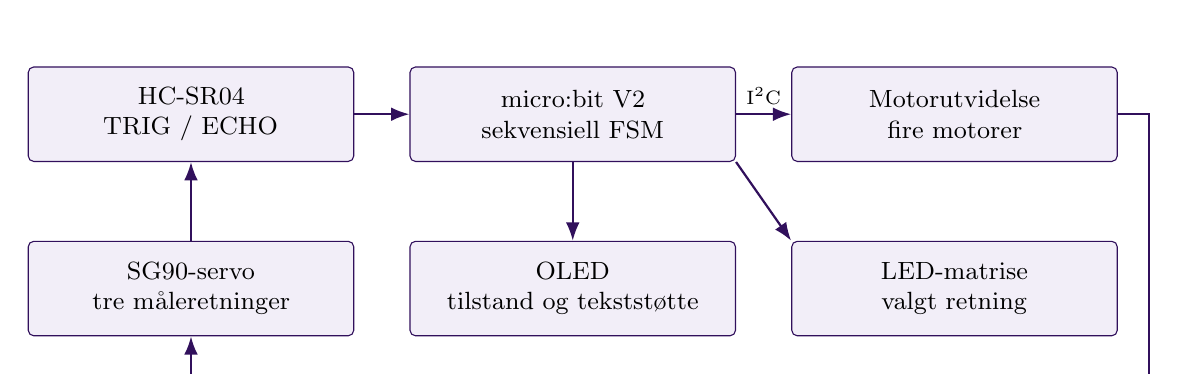
\begin{tikzpicture}[>=Latex,font=\small,
 box/.style={draw=usnpurple,rounded corners=2pt,align=center,
 fill=softpurple,minimum height=12mm,text width=39mm},
 arr/.style={->,thick,draw=usnpurple}]
\node[box] (sensor) {HC-SR04\\TRIG / ECHO};
\node[box,right=7mm of sensor] (fsm) {micro:bit V2\\sekvensiell FSM};
\node[box,right=7mm of fsm] (motor) {Motorutvidelse\\fire motorer};
\node[box,below=10mm of sensor] (servo) {SG90-servo\\tre måleretninger};
\node[box,below=10mm of fsm] (oled) {OLED\\tilstand og tekststøtte};
\node[box,below=10mm of motor] (led) {LED-matrise\\valgt retning};
\draw[arr] (sensor)--(fsm);
% Tegn pil og etikett separat for robust parsing i nyere PGF/pdfLaTeX.
\draw[arr] (fsm.east) -- (motor.west);
\node[above,font=\scriptsize]
 at ($(fsm.east)!0.5!(motor.west)$) {$\mathrm{I}^{2}\mathrm{C}$};
\draw[arr] (motor.east) -- ++(4mm,0) |- ([yshift=-6mm]servo.south) -- (servo.south);
\draw[arr] (servo)--(sensor);
\draw[arr] (fsm)--(oled);
\draw[arr] (fsm.south east)--(led.north west);
\end{tikzpicture}
\caption{Signal- og kommandoflyt. Servo styres gjennom motorutvidelsen.
Strømforsyning og fullstendig elektrisk kobling er utelatt.}
\label{fig:system}
\end{figure}

\section{Maskinvarearkitektur}
\begin{table}[htbp]
\small
\begin{tabularx}{\textwidth}{@{}P{31mm}YP{43mm}@{}}
\toprule Komponent & Tilkobling eller rolle & Dokumentasjonsstatus\\\midrule
Micro:bit V2 & Utfører Ada-programmet; viser LED-piler. & Kode og rapportert fysisk test.\\
Mecanum-bil & Fire motorer via ekstern motorutvidelse. & Oppgitt prosjektplattform.\\
HC-SR04 & Frontsensor: TRIG P13, ECHO P1. & Generisk instans i main.adb.\\
SG90-servo & Driverens servokanal 2; kommandoer 64, 84 og 104 grader. & Kode og utviklingslogg.\\
Motorutvidelse & MicroBit.MotorDriver bruker DFR0548-driver på ekstern I\textsuperscript{2}C. & Verifisert driversti; fysisk kortrevisjon må angis.\\
OLED & Ekstern I\textsuperscript{2}C, P19/P20; adresseargument 16\#78\#. & Direkte overføringer i kode; eksakt skjermmodell uavklart.\\
Strømforsyning & Forsyning til kort, sensor, servo og motorer. & Selvstendig stabil drift ikke verifisert.\\
\bottomrule
\end{tabularx}
\caption{Maskinvare og grensesnitt i dagens program.}
\label{tab:hardware}
\end{table}

Tidligere prosjektmateriale oppgir en bakre sensor med TRIG P12/ECHO P0,
og motorplasseringen M1 bak venstre, M2 foran venstre, M3 bak høyre og M4 foran
høyre~\cite{tidligere}. Dagens applikasjon instansierer bare frontsensoren.
Bakre sensor og tidligere kanaltilordning beholdes som utviklingshistorikk;
de gir ikke dokumentasjon på aktiv bakoverbeskyttelse.

\todo{Legg inn datert foto og fullstendig koblingsskjema med fysisk kortmodell,
motorporter, sensorforsyning, felles jord og nivåtilpasning. Bekreft motorretning
for hver kanal.} DFR0548 har ifølge produsenten fire motorkanaler og
servogrensesnitt~\cite{dfr0548}; dette identifiserer ikke alene det monterte kortets revisjon.

\section{Programvarearkitektur}
Etter initialisering kjøres \kode{case Current_State} sekvensielt med
sensoravlesning, filtrering, beslutning, skjerm og motorhandling~\cite{kode}.
Tre målinger per retning gir én filtrert avstand og ett
\kode{Best_Direction}. Dataene har ikke tidsstempel eller eget gyldighetsfelt.
Null behandles som blokkert retning, uten å skille målefeil fra nær hindring.

\section{Task-arkitektur}
Originalforslaget var Sensor Task, sensordata, Control Task, ønsket bevegelse,
Motor Task og motorer, supplert med Safety Task. Forslaget er bevart i
tabell~\ref{tab:tasks}.

\begin{table}[htbp]
\small
\begin{tabularx}{\textwidth}{@{}P{31mm}Y@{}}
\toprule Foreslått task & Tiltenkt ansvar, ikke implementert som egen task\\\midrule
Sensor\_task & Periodisk innhenting av sensordata. Et mulig tillegg er gyldighet og tidsstempel.\\
Control\_task & Vurdere sensordata og bestemme bilens bevegelse.\\
Motor\_task & Utføre ønsket bevegelse ved å styre motorene.\\
Safety\_task & Håndtere kritiske situasjoner og kollisjonsfare.\\
\bottomrule
\end{tabularx}
\caption{Bevart task-forslag fra originalrapporten. Perioder og prioriteter er ikke fastsatt.}
\label{tab:tasks}
\end{table}

Ved eventuell implementasjon må tilgang til delte data og rask stopp
under skjermtegning og skanning utformes og verifiseres.

\section{Kontrollstrategi}
Originalskissen var kjøring, sensoravlesning, hinderkontroll, eventuell
unnamanøver og videre kjøring ved fri vei. FSM-en bruker nå fremoverpulser
og prioriterer frem, høyre, venstre, ikke nødvendigvis størst avstand.

\begin{table}[htbp]
\small
\begin{tabularx}{\textwidth}{@{}P{25mm}YP{38mm}@{}}
\toprule Tilstand & Faktisk handling & Neste tilstand\\\midrule
Stop & Motorstopp, status, vent 0,5 s. & Scan.\\
Scan & Motorstopp; mål høyre, frem og venstre; sentrer servo. & Verify ved fri front; Turn ved fri side; ellers Stop.\\
Turn & Roter høyre/venstre i 0,3 s med PWM 800, deretter stopp. & Verify.\\
Verify & Motorstopp; mål front på nytt etter servoventetid. & Forward ved godkjent avstand; ellers Stop.\\
Forward & Fremoverkommando med PWM 800 i 0,2 s, så stopp. & Verify.\\
Reverse\_Drive & Stopper motorene; reservert for senere rygging. & Stop; ingen ordinær overgang inn i tilstanden.\\
\bottomrule
\end{tabularx}
\caption{FSM-handlinger fra revisjon ee6df67. Ventetider er kodeverdier.}
\label{tab:fsm}
\end{table}

\section{Sanntidsdesign}
Sensorfrekvensen avhenger av tilstanden og relative \kode{delay}-setninger;
én fast periode er ikke etablert. LED-driverens timer har nominell periode
900~$\mu$s. Dette er ingen deadline for kollisjonshåndtering. Tidsanalysen
må omfatte kontrollflyt, timeraktivitet, I\textsuperscript{2}C og logging.
\todo{Velg og dokumenter tidskrav ut fra fart, sensordekning og målt oppbremsing.}

\chapter{Implementasjon}\label{ch:impl}
\section{Motorstyring}
Motorene styres gjennom \kode{MicroBit.MotorDriver.Drive}.
Applikasjonen bruker \kode{Forward}, \kode{Rotating_Right},
\kode{Rotating_Left} og \kode{Stop}. Alle fire logiske hjulparametre,
\kode{rf}, \kode{rb}, \kode{lf} og \kode{lb}, settes til 800 ved aktiv kjøring.
Fremoverpulsen varer nominelt 0,2~s og rotasjonspulsen 0,3~s, før en
stoppkommando sendes~\cite{kode}.

Dette er åpen styring med tidsbestemte kommandoer. Det er ikke implementert
fartsmåling, regulering med hjulfeedback eller måling av svingvinkel i
hovedprogrammet. Programverdien 800 kan derfor ikke oversettes til m/s eller
en bestemt rotasjonsvinkel uten kalibrering.

En kommentar før FSM-løkken sier at fremoverkjøring er deaktivert under testen.
Den kjørbare \kode{Forward}-grenen sender likevel en aktiv fremoverkommando.
Beskrivelsen her følger den kjørbare koden. Kommentaren må korrigeres ved
neste kodeendring; den er ikke en sikker avsperring av motorene.

\section{Mecanum-bevegelse}
Driveren setter motorenes retning og PWM gjennom DFR0548-komponenten.
Rotasjon frembringes ved å kjøre venstre og høyre side i motsatt retning.
Tidligere materiale oppgir individuelle motortester, og loggen fra
21.10 omtaler motorrespons og høyresving fra tidligere benkearbeid~\cite{tidligere,logg}.
Et komplett resultatark for alle kanaler og begge svingretninger mangler.
Ingen aktiv ryggemanøver eller sideveis manøver inngår i dagens FSM.

\section{Sensorimplementasjon}
Frontsensoren er instansiert som
\kode{MicroBit.Ultrasonic (MB_P13, MB_P1)}. I \kode{Scan} settes servoen til
64 grader for høyre, 84 for frem og 104 for venstre. Programmet venter
0,8~s etter hver posisjonskommando, tar tre avlesninger med 0,07~s mellomrom,
og sentrerer deretter servoen med ytterligere 0,8~s venting.

Funksjonen \kode{Median} er ikke en matematisk median. Den krever minst
to målinger i intervallet 2--200~cm som er høyst 15~cm fra hverandre.
Returverdien er den laveste verdien i samsvarende par, eller null hvis
ingen par godkjennes. Funksjonen beskrives derfor her som et konservativt
samsvarsfilter. Navnet beholdes i kodevedlegget.

Retningsvalget i \kode{Scan} godtar 45--200~cm. \kode{Verify} tester
45--400~cm, men bruker samme filter med øvre grense 200~cm. Den effektive
godkjenningsgrensen er dermed 200~cm også der. Dette er et kodefunn som
må avklares; det er ikke en sensorvalidering.

Begge timeout-grenene i ultralyddriveren er rettet med \kode{exit Polling},
slik at pollingløkkene avsluttes. Det retter den manglende avslutningen
som ble identifisert i tidligere kildegjennomgang~\cite{tidligere}.
Timeout-parametrene er fortsatt 3~ms for start og 23~ms for ekkoslutt.
Avstanden estimeres ved løkketelling med \kode{Delay_Us(58)}.
Disse innstillingene er ikke målt WCET, og nøyaktighet og tidsoppførsel
under avbrudd må fortsatt testes.

\Needspace{10\baselineskip}
\section{Ada-tasks}
Applikasjonen kjører FSM-en i hovedprosedyren, med høyst 60 tilstandssteg.
Et steg er én gjennomkjøring av én tilstandsgren; grensen betyr ikke
60 komplette kjøre- eller skannesykluser. Etter løkken sendes \kode{Stop},
status oppdateres, og programmet forblir i en venteløkke frem til reset.

Det finnes ikke egne \kode{Sensor_task}, \kode{Control_task},
\kode{Motor_task} eller \kode{Safety_task} i hovedprogrammet.
LED-driverens bakgrunnsoppdatering er en bibliotekaktivitet og endrer ikke
denne beskrivelsen av applikasjonen. Den valgte runtime er
\kode{embedded-nrf52833}; aktiv taskingprofil og øvrige runtime-aktiviteter
må bekreftes før en full planleggingsanalyse.

\section{Integrasjon}
\subsection{OLED og I2C}
Programmet initialiserer ekstern I\textsuperscript{2}C med
\kode{S100kbps}. OLED styres med direkte kommandoer og tegnmønstre i
hovedprogrammet. \kode{Show_Front} kan tegne avstand, mens
\kode{Show_Status} tegner FSM-tilstand. I denne revisjonens FSM brukes
\kode{Show_Status}; \kode{Show_Front} er definert, men ikke kalt i
den aktive løkken. Derfor er kontinuerlig avstandsvisning en tilgjengelig
kodefunksjon, ikke påvist aktiv visning under FSM-testen.

Adresseargumentet er \kode{16#78#}. Eksakt OLED-kontroller, modulvariant
og adressekonvensjon må dokumenteres før dette brukes som koblingsfasit.
I\textsuperscript{2}C-patchen konfigurerer ekstern SCL/SDA eksplisitt med
pull-up og valgt GPIO-drivemodus. Feilstatus fra OLED-overføringer logges,
men hovedprogrammet går ikke automatisk til en feilsikker tilstand ved
skjermfeil. Motor- og OLED-trafikk bruker samme eksterne kontroller.

\subsection{LED-retningspiler}
Et byggproblem oppstod da \kode{MicroBit.Display} ikke var tilgjengelig
i prosjektets full-konfigurasjon. Løsningen var å bruke
\kode{MicroBit.DisplayRT}, som er tilgjengelig gjennom
\kode{microbit_v2_full.gpr}~\cite{logg}.
\kode{Show_Direction} tegner fremoverpil, høyrepil, venstrepil eller kryss.
Pilen settes i skannetilstanden og viser FSM-ens valgte retning.
Den er ikke en kontinuerlig måling av kjøretøyets bevegelse, og en tidligere
pil kan bli stående etter en senere stopp i \kode{Verify}.

\subsection{Bygg og versjon}
Revisjon \kode{ee6df67ab8ebec4e309195324f941b61602a1a36} har meldingen
\enquote{feat: implement autonomous FSM and LED direction indicators}.
Den inkluderer \kode{main.adb}, utviklingsloggen og den rå driverpatchen.
\kode{Code/itrs.gpr} velger Ada 2022, \kode{arm-eabi} og full-prosjektet
for micro:bit V2. Alire-filen låser \kode{gnat_arm_elf} til 15.1.2 og
\kode{gnatprove} til 15.1.0. Dette dokumenterer konfigurasjonen, ikke
gjennomført SPARK-bevis~\cite{kode}.

\chapter{Sanntidsanalyse}\label{ch:rt}
\section{Oppgaver og prioriteter}
Analyseobjektet per 21.10 er en sekvensiell applikasjon med driver- og
runtime-aktiviteter i bakgrunnen. Hovedprogrammets \kode{delay}-setninger
er relative ventetider; de etablerer ikke en periodisk taskmodell.
Sensoravlesning, OLED og konsolltrafikk ligger i samme kontrollflyt og
kan påvirke når neste motorbeslutning tas.

For et senere taskdesign må man fastsette hvilke aktiviteter som er
periodiske, hvilke som utløses av hendelser, og hvordan tilgang til motorer,
sensordata og I\textsuperscript{2}C koordineres. Prioritet til sikkerhet
er et designønske inntil en konkret oppgave- og blokkeringsmodell foreligger.

\section{Perioder og deadlines}
\begin{table}[htbp]
\small
\begin{tabularx}{\textwidth}{@{}P{30mm}YP{36mm}@{}}
\toprule Aktivitet & Kjent fra kode & Formelt tidskrav\\\midrule
Frontmåling & Tre avlesninger per målegruppe; 70 ms mellom avlesninger. & \todo{Fastsett $T$ og maksimal målealder.}\\
Servoskanning & Fire ventinger à 0,8 s i Scan. & \todo{Definer maksimal tillatt skannetid.}\\
Kollisjonsreaksjon & Ny kontroll i Verify før neste fremoverpuls. & \todo{Definer $D_{\mathrm{stopp}}$ fra fysisk hendelse.}\\
Fremoverpuls & 0,2 s før stoppkommando. & Kodeparameter; ingen validert fysisk sikkerhetsgrense.\\
Rotasjonspuls & 0,3 s før stoppkommando. & \todo{Krav til sideklaring og reaksjon under rotasjon.}\\
LED-oppdatering & Driverparameter 900 $\mu$s. & Ingen egen applikasjonsdeadline fastsatt.\\
\bottomrule
\end{tabularx}
\caption{Kjente programtider og tidskrav som fortsatt må fastsettes.}
\label{tab:tider}
\end{table}

Den summerte planlagte ventingen i \kode{Scan} er
\begin{equation}
W_{\mathrm{Scan}}=4\cdot0{,}8+3\cdot2\cdot0{,}07=3{,}62\ \mathrm{s}.
\label{eq:scan}
\end{equation}
Tilsvarende er ventingen i én \kode{Verify}-gren
$W_{\mathrm{Verify}}=0{,}8+2\cdot0{,}07=0{,}94$~s.
Dette er statiske summer av venteargumenter, ikke observerte kjøretider,
WCET eller totale grenstider. Sensor-, buss- og loggtid kommer i tillegg.
Motorene er kommandert stoppet under skanning og verifisering.

\section{WCET}
Ingen dokumentert WCET-måling foreligger. Timeout-konstantene i driveren
kan ikke uten videre summeres og erklæres som WCET. Oppløsning på klokke,
løkkeoverhead, driverkall og bakgrunnsaktivitet må inngå i begrunnelsen.
Aktiv polling bruker prosessor, mens en Ada-venting normalt suspenderer
den kallende utførelsen. Det er derfor nødvendig å skille prosessortid fra
forløpt tid i tilstandssekvensen.

En måleprotokoll bør knytte hver måling til firmwarehash, kompilatorvalg,
patch, strømforsyning og aktiv logging. Mål inngang og utgang av kritiske
grener, ekkofeil og motoroverføring med en egnet tidskilde, og vurder
instrumenteringens egen påvirkning. Maksimal observert tid er et måleresultat;
en garantert verstefallsgrense krever i tillegg dekkende analyse.
\todo{Før inn målemetode, antall forsøk, rådata, maksimalt observert tid og begrunnet grense.}

\section{Response Time Analysis}
For et fremtidig oppgavesett med én prosessor, faste prioriteter,
preemptiv planlegging, begrensede kjøretider og uten selvsuspensjon kan
en grunnmodell uten release-jitter skrives som~\cite{rta}
\begin{equation}
R_i^{(k+1)}=C_i+B_i+
\sum_{j\in hp(i)}\left\lceil\frac{R_i^{(k)}}{T_j}\right\rceil C_j,
\qquad R_i^{(0)}=C_i+B_i.
\label{eq:rta}
\end{equation}
Her er $hp(i)$ oppgavene med høyere prioritet, og $B_i$ en begrunnet
blokkeringsgrense. Iterasjonen fortsetter til et fastpunkt er funnet eller
deadline overskrides. Jitter, avbrudd og eventuelle suspensjoner krever
egnet utvidelse eller en konservativ modell. Ligning~\eqref{eq:rta} er en
metodebeskrivelse og anvendes ikke numerisk på dagens FSM.

\begin{table}[htbp]
\small
\begin{tabularx}{\textwidth}{@{}Ycccccc@{}}
\toprule Foreslått aktivitet & $T_i$ & $D_i$ & $C_i$ & $B_i$ & Prioritet & $R_i$\\\midrule
Sensor & TODO & TODO & TODO & TODO & TODO & TODO\\
Kontroll & TODO & TODO & TODO & TODO & TODO & TODO\\
Motor & TODO & TODO & TODO & TODO & TODO & TODO\\
Sikkerhet & TODO & TODO & TODO & TODO & TODO & TODO\\
\bottomrule
\end{tabularx}
\caption{Analyseark for en eventuell senere taskimplementasjon. Alle verdier er uavklarte.}
\label{tab:rta}
\end{table}

\section{Verifisering av deadlines}
For dagens sekvensielle løsning må det lages en ende-til-ende-modell fra
en fysisk hindring til sensorregistrering, beslutning, motoroverføring og
faktisk stopp. Et mulig kravgrunnlag er
\begin{equation}
d_{\mathrm{krav}}\ \geq\ v_{\max}L_{\mathrm{reaksjon}}+
d_{\mathrm{brems}}+m,
\label{eq:stopp}
\end{equation}
der $L_{\mathrm{reaksjon}}$ inkluderer venting til neste relevante måling,
og $m$ er en begrunnet margin. Ingen av størrelsene er målt her.
45~cm kan derfor ikke begrunnes som tilstrekkelig sikkerhetsavstand.
Bevegelige hindringer krever også at relativ bevegelse og sensordekning
tas med. \textbf{RT1--RT3 er ikke dokumentert oppfylt per rapportdato.}

\chapter{Tester og resultater}\label{ch:test}
\section{Testresultater}
Resultatgrunnlaget er utviklingsloggen fra 21.10.2026, tidligere rapportarbeid
og kildekontroll av \kode{ee6df67}~\cite{logg,tidligere,kode}.
Det er ikke kjørt nye firmwarebygg eller fysiske tester ved denne
rapportoppdateringen. \emph{Bestått i logg} nedenfor er et rapportert resultat,
ikke en uavhengig gjentakelse.

\begin{table}[htbp]
\small
\begin{tabularx}{\textwidth}{@{}P{47mm}YP{39mm}@{}}
\toprule Test eller kontroll & Resultat & Bevis og begrensning\\\midrule
Ada-kompilering og linking & Bestått i logg. & Utviklingslogg 21.10; rå bygglogg ikke vedlagt.\\
Generering av main.hex & Bestått i logg. & Kobling til eksakt binærhash mangler.\\
Flashing til micro:bit V2 & Bestått i logg. & Ikke gjentatt ved rapportoppdateringen.\\
LED-retningsvisning & Fungerer, bekreftet av utvikler i logg. & Ikke systematisk test av alle symboler og overganger.\\
Stopp, skanning, motorrespons og høyresving & Tidligere benkeobservasjoner rapportert. & Ikke alle gjentatt 21.10; rå protokoll mangler.\\
Autonom gulvkjøring uten USB & Ikke ferdig verifisert. & Stabil strømforsyning og helhetlig kjøring gjenstår.\\
Kildekontroll mot ee6df67 & Hovedprogram samsvarer med revisjonen. & Bekrefter kodeinnhold, ikke fysisk oppførsel.\\
Driverpatch & Reverse-kontroll passer lokal drivertilstand. & Statisk patchkontroll; ingen ny firmware- eller feiltest.\\
\bottomrule
\end{tabularx}
\caption{Rapporterte testresultater og separate kildekontroller.}
\label{tab:resultater}
\end{table}

\section{Funksjonelle tester}
Tabell~\ref{tab:testplan} definerer videre kontroller. Ingen av radene
skal leses som bestått uten en datert protokoll. Protokollen må oppgi
revisjon, faktisk oppsett, forventning, observasjon og eventuelle avvik.

{\small
\begin{longtable}{@{}P{10mm}P{16mm}P{64mm}P{54mm}@{}}
\caption{Testplan knyttet til opprinnelige krav. Status er planlagt eller ikke fullført.}
\label{tab:testplan}\\
\toprule ID & Krav & Fremgangsmåte & Akseptkriterium og status\\\midrule
\endfirsthead
\toprule ID & Krav & Fremgangsmåte & Akseptkriterium og status\\\midrule
\endhead
F1 & SR3 & Løft hjulene; identifiser hver motor og begge rotasjonsretninger.
& Riktig fysisk hjul og retning for alle kanaler. Full protokoll mangler.\\
F2 & FR2, SR4 & Sammenlign rå og filtrerte målinger med kjente avstander og ulike målflater.
& \todo{Fastsett toleranse, antall forsøk og gyldighetskriterier.}\\
F3 & FR2--FR4 & Test fri front, kun fri høyre, kun fri venstre og alle retninger blokkert.
& Rekkefølgen frem, høyre, venstre, stopp stemmer med kode og LED. Ikke fullverifisert.\\
F4 & FR3, FR4 & Fremprovoser manglende ekko, fast høyt/lavt ekko og uenige avlesninger.
& Avlesning avsluttes; ingen ny kjøreordre ved ugyldig data. Måles og protokollføres.\\
F5 & FR4--FR6 & Test hver FSM-overgang, korte fremoverpulser, begge svinger og blokkering etter sving.
& Forventet neste tilstand og motorhandling. Systematisk overgangsdekning mangler.\\
F6 & FR1, FR6 & Kjør kontrollert på gulv med selvstendig strømforsyning og kjente hindringer.
& \todo{Fastsett bane, hastighet, varighet og antall gjentakelser.} Ikke ferdig verifisert.\\
F7 & FR1 & Kjør til testgrensen og observer motorer og status.
& Stopp etter 60 tilstandssteg og ingen ny kjøring før reset. Ikke fysisk protokollført.\\
F8 & SR1, SR3 & Kontroller forsyning ved samtidig servo- og motorbelastning uten USB.
& \todo{Fastsett spenningsgrenser og belastningsforløp.} Stabil drift uverifisert.\\
\bottomrule
\end{longtable}}

\section{Sanntidstester}
Reaksjonstestene må dekke at hindringen oppstår rett etter en måling, mens
en fremoverpuls pågår, og under rotasjon. Tiden til motorenes stoppkommando
og tiden til fysisk stopp må registreres hver for seg. Tidsmåling ved bare
én gunstig FSM-posisjon gir ikke en verstefallsgrense.

\begin{table}[htbp]
\small
\begin{tabularx}{\textwidth}{@{}P{10mm}P{18mm}Y@{}}
\toprule ID & Krav & Måling som gjenstår\\\midrule
T1 & RT1 & Mål intervall og alder for relevante sensorverdier i alle tilstandsforløp.\\
T2 & RT2 & Mål fysisk hinderhendelse til stoppkommando og til stillstand, også ved ugunstig fase.\\
T3 & RT3 & Mål kritiske kodegrener, ekkotimeout, I\textsuperscript{2}C-overføring og interferens.\\
T4 & RT2, RT3 & Gjenta med skjerm og logging aktiv, ved bussfeil og realistisk strømforsyning.\\
\bottomrule
\end{tabularx}
\caption{Planlagte tidsmålinger. Deadlines og måledata er fortsatt TODO.}
\end{table}

\section{Resultater}
\begin{table}[!ht]
\small
\begin{tabularx}{\textwidth}{@{}YP{38mm}P{49mm}@{}}
\toprule Størrelse & Rapportert verdi & Tolkning\\\midrule
Flashforbruk & 191\,324 byte (36,49\,\%) & Oppgitt i logg for siste bygg.\\
RAM-forbruk & 15\,600 byte (11,90\,\%) & Oppgitt byggverdi; ikke målt verstefall for stakk.\\
Byggetid & 2,04 s & Tid for byggprosessen; ikke programmets responstid.\\
Kompilatoradvarsler & Fire ultralydrelaterte advarsler & Ordrett advarseltekst og konsekvens må dokumenteres.\\
\bottomrule
\end{tabularx}
\caption{Byggopplysninger fra utviklingsloggen~\cite{logg}. Rå logg og binærhash mangler.}
\label{tab:bygg}
\end{table}

Disse resultatene dokumenterer fremdrift i integrasjon og visning.
De dokumenterer ikke kjørehastighet, sensorpresisjon, sikker stopplengde,
kontinuerlig autonom drift eller at deadlines er overholdt.

\clearpage
\section{Feilsøking og videreutvikling 23.10.2026}\label{sec:utvikling23}
Denne daterte oppdateringen supplerer den bevarte rapporten. Den skiller
mellom tidligere utviklerobservasjoner, avleste data fra fysisk micro:bit,
automatiserte tester og forhold som fortsatt krever praktiske forsøk.
Arbeidet tok utgangspunkt i lokale endringer etter \kode{ee6df67}; disse
ble sikkerhetskopiert før endring. Ingen endringer er publisert til GitHub.

\subsection{Oppstartsregresjon: observasjon, årsak og isolert retting}
Den rapporterte feilen var at OLED viste ADAptive, mens servo og motorer
sto stille etter utvidelsen med ytterpunkter. Før flashing ble hele
flashminnet på 524\,288 byte lest ut. Programområdet samsvarte byte for
byte med den lokale binærfilen. Prosessoren sto i feilhandleren ved
\kode{PC=0x16c08}; \kode{xPSR=0x21000006} viste UsageFault, og
\kode{CFSR=0x00040000} viste ugyldig exception return.

Den opprinnelige primærstakken var 4096 byte. Kompilatorens stakkrapport
viste at \kode{Main} alene reserverte 3424 byte før underkall og
avbruddskontekst. Den avleste prosess-stakkpekeren
\kode{0x200031b0} lå under stakkens nedre grense \kode{0x20003260},
inne i området reservert til avbruddsstakken. Samlet dokumenterer dette
stakkoverløp som forklaring på oppstartsregresjonen; det er ikke
dokumentasjon på en feil i én bestemt servovinkel.

En isolert endring økte stakken til 16\,384 byte. Dette ble satt som
linkerparameter:\par
\kode{--defsym=__stack_size=16384}.\par
Etter flashing passerte programmet
OLED-initialisering, startet autonom FSM og utførte 5P/7P-skanning.
Feilregisteret var da null. Utvikler bekreftet fysisk servobevegelse og at
34--134\textdegree{} er mekanisk kontrollert. Dette bekrefter oppstartsrettingen,
men ikke full autonom kjøring. Etter moduldelingen rapporterer kompilatoren
912 byte for \kode{Main}, merket dynamisk. Dette er et bidrag fra én
funksjon, ikke en fullstendig øvre stakkgrense. En markørtest under et
15-sekunders forløp med verifikasjon og skanning viste 1976 byte brukt
av primærstakken; 14\,408 byte i bunnen beholdt markøren. Dette er
en observert høytvannsverdi, ikke en verstefallsgrense.

\subsection{Moduler, navigasjon og sikkerhetskontroller}
Den aktive applikasjonen er fortsatt sekvensiell. Egen kode for
policy, FSM, sensorer, navigasjon, motorutgang, skjerm og stoppforespørsel
erstatter den store lokale kontrollblokken. Ingen sensor-, kontroll- eller
sikkerhetstasks er innført. FSM-en bruker nå \kode{Stopped}, \kode{Verify},
\kode{Cruise}, \kode{Scan}, \kode{Turn} og en låst \kode{Fault}.
Det historiske \kode{Reverse_Drive} var allerede bare stopp og er ikke
en aktiv manøver i den nye implementasjonen.

\begin{figure}[htbp]
\centering
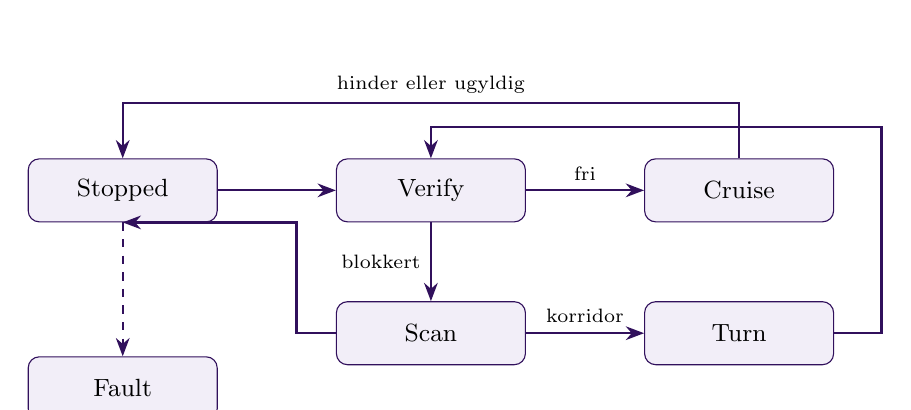
\begin{tikzpicture}[
 node distance=10mm and 15mm,
 box/.style={draw=usnpurple,rounded corners,fill=softpurple,
  minimum width=24mm,minimum height=8mm,font=\small},
 arr/.style={-{Stealth},thick,draw=usnpurple}]
\node[box] (stop) {Stopped};
\node[box,right=of stop] (verify) {Verify};
\node[box,right=of verify] (cruise) {Cruise};
\node[box,below=of verify] (scan) {Scan};
\node[box,right=of scan] (turn) {Turn};
\node[box,below=17mm of stop] (fault) {Fault};
\draw[arr] (stop)--(verify);
\draw[arr] (verify)--node[above,font=\scriptsize]{fri} (cruise);
\draw[arr] (verify)--node[left,font=\scriptsize]{blokkert} (scan);
\draw[arr] (scan)--node[above,font=\scriptsize]{korridor} (turn);
\draw[arr] (turn.east)--++(6mm,0)|-([yshift=4mm]verify.north)--(verify.north);
\draw[arr] (cruise.north)--++(0,7mm)-|node[pos=.25,above,font=\scriptsize]{hinder eller ugyldig} (stop.north);
\draw[arr] (scan.west)--++(-5mm,0)|- (stop.south);
\draw[arr,dashed] (stop)--(fault);
\end{tikzpicture}
\caption{Forenklet aktiv FSM. Etter sving kreves ny verifikasjon.
Feil og stoppforespørsel låser kjøringen i Fault; uventede hendelser gir stopp.}
\label{fig:fsm23}
\end{figure}

Frontsensoren sentreres på 84\textdegree{}. Før start kreves gyldige
front- og sidemålinger. Ved fremoverkjøring beholdes motorutgangen mellom
kontrollene i stedet for fem adskilte pulser. Akustiske triggere holdes
minst 65 ms fra hverandre. Rekkefølgen under bevegelse er front, venstre,
front, høyre. Ugyldige råmålinger og frontavstand på høyst 45 cm
utløser stopp før logging eller neste sensorlesing. Sideterskelen er
15 cm under fremoverkjøring og 25 cm under sving; fronten krever også
mer enn 25 cm før sving. Stasjonær filtrering krever at alle tre målinger
er gyldige og minst to stemmer innen 15 cm. Minste verdi beholdes slik
at en kort hindermåling ikke forkastes til fordel for to store verdier.
Gyldig område er 2--200 cm; 0 cm gir aldri kjøretillatelse.

5P bruker 60, 72, 84, 96 og 108\textdegree{}. Ved manglende godkjent
retning følger 7P ved 54, 64, 74, 84, 94, 104 og 114\textdegree{}.
Når 7P er blokkert, gir ytterpunktene 34 og 134\textdegree{} ekstra
informasjon. De kan ikke alene oppheve en blokkert korridor.
En utvidet svingbeslutning krever to like godkjente 7P-valg og ny kontroll
av front og begge sider før motorstart. Bekreftelsen forbrukes ved bruk.

Utvikler oppga bredde 16 cm, lengde 23 cm og omtrent 10 cm
sensorforskyvning. En foreløpig geometrisk test krever at
\(2d_{\min}\sin(\Delta\theta/2)\geq 16+2\cdot5=26\) cm over den
skannede sektoren. Det tilsvarer bilens bredde med 5 cm tillegg på hver side.
Dette avviser smale vinkelåpninger selv om enkeltstrålene passerer 45 cm.
Sparsom ultralydskanning beviser likevel ikke at hele arealet er tomt.
Sensorplassering, blindsoner, svingbane og marginer må verifiseres fysisk.

Motorutgangen kontrollerer I\textsuperscript{2}C-status. Sendefunksjonen
i \kode{nrf-twi.adb} var tidligere uten aktiv timeout; den nye aktive
sendestien har tidsgrense både for data og STOP-hendelse. Motortransaksjoner
bruker 20 ms som programparameter. Ved feil forsøkes stopp, og videre
kjøring låses. En brutt buss kan hindre at selve stoppkommandoen når
motorbrettet; fysisk frakobling av motorstrøm er derfor fortsatt nødvendig
ved benketest. Knapp B ber om låst stopp, kontrollert mellom sensorlesingene.

\subsection{Ultralydadvarsler og tidsmessig avgrensning}
Advarslene ved de tidligere linjene 70 og 92 skyldtes polling av
GPIO-objektet \kode{Echo}, som ikke ble endret i løkkekroppen.
Den undersøkte lokale koden hadde allerede eksplisitte timeout-utganger.
Advarselen var derfor ikke bevis for en uendelig løkke eller årsaken til
den observerte UsageFault-feilen. Pollingen er skrevet om med klokken
direkte i løkkebetingelsen og retur av 0 ved utløpt tid. Den bruker
3 ms for venting på ekkostart og 23 ms for ekkoslutt. Disse er
programmerte grenser; pollingoverskridelse, avbrudd og klokkeavhengighet
må inngå i en faktisk WCET-analyse. Det nye bygget gir ingen av de tidligere
ultralydadvarslene.

Med normal tidsdrift gir triggerplanen omtrent 130 ms mellom fronttriggere
og 260 ms mellom triggere fra samme sidesensor under bevegelse. Dette er
analyse av kontrollflyten, ikke målt responstid eller deadlinebevis.
Stopplengden må fortsatt beregnes fra målt hastighet, målealder,
behandling, utgangsforsinkelse og fysisk bremsing. Forelesningene skiller
responstid fra funksjonell korrekthet og beskriver fail-safe som å bevare
integritet selv om driften avbrytes~\cite{forelesninger2026}.

\subsection{Testgrunnlag og gjenstående demonstrasjon}
\begin{longtable}{@{}P{36mm}P{39mm}P{71mm}@{}}
\caption{Daterte kontroller 23.10.2026. Resultatene gjelder bare oppgitt omfang.}
\label{tab:tester23}\\
\toprule Kontroll & Resultat & Bevis eller avgrensning\\\midrule
\endfirsthead
\toprule Kontroll & Resultat & Bevis eller avgrensning\\\midrule
\endhead
Backup og firmwareproveniens & Bestått & 51 lokale filer med manifest, Git-patcher og full flashkopi. Programområdet samsvarte med lokalt bygg.\\
Isolert stakkretting & Bestått benkeobservasjon & Oppstart og FSM kom videre; CFSR var 0. Fysisk servo bekreftet av utvikler.\\
Policy og FSM på vertsmaskin & 1729 kontroller bestått & Faktiske Ada-moduler kjørt med native GNAT; ugyldige målinger, terskler, korridorbredde, retningsstabilitet og overganger.\\
Modulært firmwarebygg & Bestått & \kode{python tools/mb.py build}; 215\,748 byte flash og 29\,000 byte SRAM reservert. ELF/HEX/BIN generert.\\
Modulær benketest & Gjennomført, blokkert scene & Front omtrent 25 cm, venstre 100--103 cm og høyre 16 cm. 5P/7P/1P utført; 0-målinger ga ingen kjøreordre. CFSR var 0.\\
Tidligere fempulsforsøk & Utvikleropplysning & Fem pulser på 0,45 s ved PWM 800, stopp rundt 45 cm og 5P/7P-observasjoner er ikke gjentatt som samme test i denne økten.\\
Yttergrenser servo & Bekreftet av utvikler & 34--134\textdegree{} oppgitt mekanisk fritt. Ingen egen vinkelmåling eller momenttest.\\
Fremover og stopp med målflater & Bekreftet benketest & To kjørekommandoer; stopp ved venstre=0 og front=44 cm. Fysisk hjulrespons bekreftet av utvikler.\\
Autonom gulvkjøring & Gjenstår & Begge svinger, fysisk stopplengde, sidehindringer og strømforsyning uten USB må testes systematisk.\\
Feilinjeksjon og WCET & Gjenstår & Fast ekko, brutt I\textsuperscript{2}C-buss, knapp B under bevegelse og verstefallstid er ikke fysisk fullverifisert.\\
\bottomrule
\end{longtable}

En separat benketest etter at måleområdene var frigjort ga front=0,
venstre=0 og høyre=67 cm. Systemet forble blokkert selv om ytterpunktene
ga 55 og 76 cm. Det ble ikke gitt fremoverkommando i dette forsøket.

Etter oppsett med målflater ga en ny benketest gyldige verdier på
front=64, venstre=63 og høyre=75 cm og deretter fremoverkommando ved
PWM 800. Loggen viste stopp ved ugyldig venstremåling og i neste
forsøk ved front=44 cm. Utvikler bekreftet fysisk at hjulene dreide
fremover og stoppet. En gjentatt test ga også fremoverkommando og stopp ved venstre=0.
Venstresensoren ga både stabile avstander rundt
63--71 cm og periodiske 0-verdier. Årsaken til disse bortfallene er
ikke fastslått; strøm, kontaktforbindelser, målflate og akustisk
interferens må undersøkes uten å svekke målereglene.

I dette siste 15-sekunders forsøket viste stakkmarkøren 2240 byte
brukt og 14\,144 byte urørt. Ingen UsageFault ble registrert. Ved
avslutning ble stoppforespørselen satt, og indikatoren for aktiv
motorkommando var null. Det er en kontroll av programtilstand og
kommandoer, ikke en måling av hjulhastighet eller fysisk bremselengde.

Det tidligere eksemplet med venstre 6--7 cm og høyre 41--42 cm og
7P-verdiene 64\textdegree{}=46, 74\textdegree{}=21,
84\textdegree{}=21--22, 94\textdegree{}=22--23,
104\textdegree{}=23 og 114\textdegree{}=162 cm kommer fra
oppdragsbeskrivelsen. Disse er tidligere enkeltobservasjoner, ikke en
ny kalibreringsserie. En slik scene gir ikke en sammenhengende godkjent
korridor. De nye råloggene og driverpatchen ligger sammen med
utviklingsloggen i Git-arbeidsmappen; eldre kodevedlegg er beholdt med
sin opprinnelige revisjonsangivelse.

\clearpage
\section{Stasjonær sensorstudie 23.10.2026}\label{sec:sensorstudie23}
Økten prioriterte sensorstabilitet fra revisjon \kode{02b542f}, etter
sikkerhetskopiering. De to nye måleseriene nedenfor supplerer de
tidligere kjøreobservasjonene i avsnitt~\ref{sec:utvikling23}.

\subsection{Oppsett, hypoteser og kontrollert innsamling}
Bruker bekreftet at motorstrømmen var frakoblet, mens USB og sensorer var
strømforsynt. En separat Ada-applikasjon initialiserer motorutgangen med
stopp og sentrerer servoen til 84\textdegree{}. Den inneholder ingen kall
til kjørefunksjonen. Etter siste måling sendes stopp igjen, og programmet
venter uten nye bevegelseskommandoer. Dette er en fysisk sensortest,
ikke en test under motorbelastning.

\begin{table}[htbp]
\centering\small
\caption{Pinnetilordning i diagnostikken og dagens navigasjonskode.}
\begin{tabular}{lll}\toprule
Sensor & TRIG & ECHO \\\midrule
Front & P13 & P1 \\
Venstre & P14 & P2 \\
Høyre & P15 & P8 \\\bottomrule
\end{tabular}
\end{table}
Bruker oppga to motstander på 1 k\(\Omega\) og 1,2 k\(\Omega\) per
ECHO-spenningsdeler. Plasseringen er ikke fysisk bekreftet. Et gjenfunnet
eldre diagram gjelder én sensor og andre motstandsverdier; det er derfor
ikke brukt som bekreftelse på dagens krets. Diagrammet brukte dessuten
P2 og P14 til LED. Bruker bekreftet etter forsøkene at bare venstre
ultralydsensor bruker disse pinnene. Hypotesen om delt LED-last legges
derfor til side; motstandsrekkefølgen er fortsatt uavklart.

Databladet anbefaler mer enn 60 ms mellom målesykluser\cite{hcsr04}.
Diagnostikken utløser bare én sensor om gangen. Hver serie har følgende
faste rekkefølge: 40 runder front--venstre--høyre med 65 ms mellom globale
utløsninger, 40 tilsvarende runder med 100 ms, deretter 40 målinger på
venstre alene med hvert intervall. Totalt blir dette 320 avlesninger per
serie. En bestemt sensor måles dermed sjeldnere enn det globale
triggerintervallet når alle tre er aktive.

Serie 1 brukte 3 ms frist for ECHO-stigning. Tidsdata viste at gyldige
venstreekko nærmet seg denne fristen. Serie 2 økte derfor bare denne
diagnostikkfristen til 10 ms. Begge hadde 23 ms frist for at en påbegynt
puls skulle avsluttes. Ved oppstart av hver avlesning kontrolleres også
om ECHO allerede er høyt. Feilkodene skiller manglende stigning,
manglende fall, allerede høyt signal og avstand utenfor 2--200 cm.
En timeout gir aldri en brukbar fri avstand.

\begin{figure}[htbp]
\centering
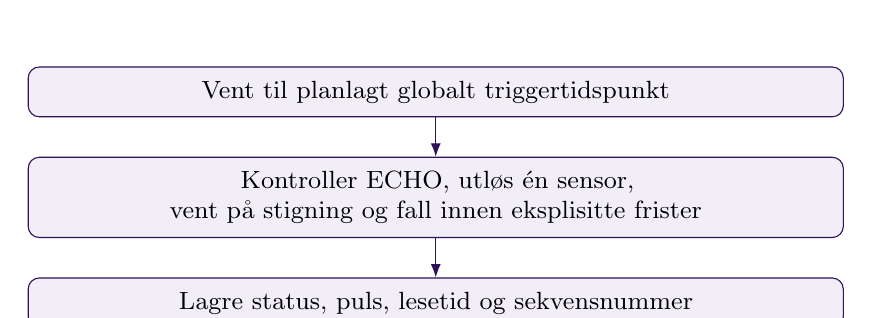
\begin{tikzpicture}[node distance=5mm,
 s/.style={draw=usnpurple,rounded corners,fill=softpurple,
 text width=10cm,align=center,font=\small,inner sep=5pt}]
\node[s] (wait) {Vent til planlagt globalt triggertidspunkt};
\node[s,below=of wait] (read) {Kontroller ECHO, utløs én sensor,\par
 vent på stigning og fall innen eksplisitte frister};
\node[s,below=of read] (log) {Lagre status, puls, lesetid og sekvensnummer};
\draw[-{Latex},usnpurple] (wait)--(read);
\draw[-{Latex},usnpurple] (read)--(log);
\end{tikzpicture}
\caption{Sekvensiell, stasjonær måleprotokoll. Motorene holdes stoppet.}
\end{figure}

\subsection{Modeller og måleusikkerhet}
Nominell avstand fra pulsbredde er
\begin{equation}
 d_{\mathrm{cm}}=\frac{t_{\mathrm{puls},\mu s}}{58}.
\end{equation}
Dette er databladets omregningsmodell\cite{hcsr04}, ikke dokumentert
nøyaktighet for det aktuelle oppsettet. Den nye rene Ada-modulen
\kode{Adaptive_Range_Model} implementerer omregningen, gyldig
arbeidsområde og spenningsdelerberegningen. Diagnostikken lagrer både
klokkebasert pulsbredde og den opprinnelige løkketelleren.

Inspeksjon av runtime-filen \kode{s-bbbosu.adb} viser at
\kode{Ada.Real_Time.Clock} bygger på RTC ved 32\,768 Hz. Ett klokketrinn
er derfor omtrent 30,5 \(\mu\)s, tilsvarende 0,526 cm i modellen.
Polling av ECHO, avrunding og avbrudd kommer i tillegg. Mikrosekunitsnavnet
i loggen betyr ikke oppløsning på ett mikrosekund. Den eldre
\kode{Delay_Us}-rutinen bruker en håndjustert NOP-løkke. Forskjellen
mellom de to avstandsestimatene kan undersøkes, men ingen av dem er
kalibrert mot kjente avstander i disse seriene.

For spenningsdeleren gjelder
\begin{equation}
 V_{\mathrm{signal}}=V_{\mathrm{ECHO}}
 \frac{R_{\mathrm{GND}}}{R_{\mathrm{serie}}+R_{\mathrm{GND}}}.
\end{equation}
Ved antatt ECHO på 5 V gir 1 k\(\Omega\) i serie og 1,2 k\(\Omega\)
til GND omtrent 2,73 V. Motsatt plassering gir omtrent 2,27 V.
Micro:bit dokumenterer \(V_{IH,\min}=0{,}7V_{DD}\)\cite{pins}; ved
antatt \(V_{DD}=3{,}3\) V blir dette 2,31 V. Den motsatte plasseringen
kan dermed mangle garantert margin for logisk høy. Dette regnestykket
bekrefter verken dagens motstandsrekkefølge, faktisk spenning eller
årsaken til venstresensorens feil. Resistortoleranse og forsyningsvariasjon
må også undersøkes.

For gyldige målinger beregner analyseverktøyet gjennomsnitt, median og
utvalgsstandardavvik. Med en faktisk oppmålt referanse \(\hat d_i\)
beregnes også
\begin{align}
 \operatorname{bias}&=\frac1n\sum_{i=1}^{n}(d_i-\hat d_i),\\
 \operatorname{MAE}&=\frac1n\sum_{i=1}^{n}|d_i-\hat d_i|,\\
 \operatorname{RMSE}&=\sqrt{\frac1n\sum_{i=1}^{n}(d_i-\hat d_i)^2}.
\end{align}
Referanseavstander ble ikke oppgitt for disse seriene. Feilmetrikkene
lagres derfor som \kode{null}. Gjennomsnittet brukes ikke som en oppdiktet
fasit. Ugyldige målinger inngår i feilandelens nevner, men aldri som
0 cm i gjennomsnittet.

\subsection{Resultater fra to fysiske serier}
Begge seriene fullførte med 320 sammenhengende sekvensnumre og
sluttmelding om stopp. Av 640 avlesninger var
front og høyre gyldige i alle sine 160 forsøk hver. Venstre ga 36 av 160
gyldige avlesninger i serie 1 og 115 av 160 i serie 2.

\begin{table}[htbp]
\centering\small
\caption{Venstre kanal, 40 avlesninger per fase. Gyldighet er
diagnostikkens status, ikke bekreftet avstandsnøyaktighet.}
\begin{tabular}{llrrrr}\toprule
Serie & Fase & Gyldige & Ugyldige & Andel ugyldige & \(s\), cm \\\midrule
1 & Alle, 65 ms &16&24&60,0\%&4,52\\
1 & Alle, 100 ms&10&30&75,0\%&5,66\\
1 & Bare venstre, 65 ms&5&35&87,5\%&2,90\\
1 & Bare venstre, 100 ms&5&35&87,5\%&2,13\\\midrule
2 & Alle, 65 ms&29&11&27,5\%&24,15\\
2 & Alle, 100 ms&28&12&30,0\%&23,06\\
2 & Bare venstre, 65 ms&30&10&25,0\%&25,88\\
2 & Bare venstre, 100 ms&28&12&30,0\%&23,54\\\bottomrule
\end{tabular}
\label{tab:left-sensor23}
\end{table}

\begin{table}[htbp]
\centering\small
\caption{Deskriptive avstander i fasen med alle sensorer og 65 ms
globalt intervall. Hver rad har 40 forsøk; spredning gjelder gyldige ekko.}
\begin{tabular}{llrrrr}\toprule
Serie & Sensor & Gyldige & Snitt, cm & Median, cm & \(s\), cm \\\midrule
1&Front&40&80,47&82,09&5,37\\
1&Venstre&16&82,08&82,35&4,52\\
1&Høyre&40&70,03&69,98&0,56\\
2&Front&40&80,31&82,60&6,35\\
2&Venstre&29&54,40&55,78&24,15\\
2&Høyre&40&70,02&69,98&0,14\\\bottomrule
\end{tabular}
\end{table}

I serie 1 var alle 124 ugyldige venstremålinger manglende ECHO-stigning.
Serie 2 hadde 44 slike feil og én avstand utenfor arbeidsområdet.
Maksimal observert lesetid var 7935 \(\mu\)s i serie 1 og
10\,071 \(\mu\)s i serie 2. Disse er observerte verdier fra en avgrenset
stasjonær test, ikke beviste WCET-grenser eller maksimal
hindring-til-motorstopp-responstid.

\subsection{Filterforsøk og vurdering av årsak}
To analysekandidater bruker ikke-overlappende tripler per fase og sensor.
Medianvarianten krever tre gyldige ekko. Den konsistente
minimumsvarianten krever i tillegg høyst 15 cm spenn og beholder den
nærmeste avstanden. Begge avviser en trippel med ugyldig måling.
Én restmåling per gruppe på 40 inngår ikke i trippelanalysen.
Serie 1 ga ingen aksepterte venstretripler for noen kandidat. Et filter
kan altså ikke gjenopprette pålitelig avstand fra disse hullene.
Kandidatene erstatter ikke den aktive navigasjonens filter.

Økt stigningsfrist ga flere mottatte ekko, men også langt større
avstandsspredning på venstre. Dette er ikke tilstrekkelig grunnlag for
å ta 10 ms inn som en ferdig retting i navigasjonen. Isolert måling
eller 100 ms intervall fjernet heller ikke feilen i disse seriene.
Fast faserekkefølge og manglende uavhengig kontroll av målscenen
begrenser årsaksslutninger. Dårlig spenningsmargin, kontaktfeil,
modulvariant og refleksjoner står fortsatt som
hypoteser. Motorstøy er ikke undersøkt med motorene i drift.

Neste forsøk bør begynne med en oppmålt, stor målflate 60 cm fra
venstre sensor og fysisk bekreftelse av
spenningsdeleren. Deretter kan venstre/høyre sensormodul byttes med
strømmen av og bare én variabel endres om gangen. Måleserier ved
20, 30, 45, 60, 100 og 150 cm er protokollført som videre arbeid;
de er ikke gjennomført eller presentert som resultater.

\subsection{Programvarekontroll, sporbarhet og sanntidsteori}
De 1729 eksisterende Ada-kontrollene besto. En ny vertsbasert Ada-suite
bestod 24 kontroller av pulsmodell, grenseverdier, ugyldige inndata og
betinget spenningsmargin. Analyseverktøyet besto 16 Python-enhetstester
med syntetiske data, blant annet kjente MAE/RMSE-verdier,
feilinjeksjon i CSV, sekvenskontroll og ugyldighetsveto. Antallet
Ada-kontroller er ikke antall fysiske forsøk eller dekningsprosent.
Både navigasjonsfirmware og separat diagnostikk ble bygget.

Sanntidsfaget definerer responstid som tiden fra inngang til nødvendig
utgang, og beskriver fail-safe som bevart integritet med midlertidig
stans\cite[PDF-s.~20 og 74]{forelesninger2026}. En sensorrutines
lesetid alene dekker derfor ikke robotens reaksjonstid. Protokollen
opprettholder sikker stopp når nødvendig informasjon er ukjent.
Ingen nye påstander om fysisk svingklarering, stopplengde, PID,
IMU-fusjon eller full autonom gulvkjøring følger av denne studien.

Rapportprosjektet inneholder begge rådatafiler (\kode{sensor-run-01.csv}
og \kode{sensor-run-02.csv}), tilhørende JSON-analyser og
\kode{SENSORPROTOKOLL.md}. Git-repoets evidensmappe bevarer dessuten
seriellogger, firmwarehash, kildeøyeblikksbilder og bygg-/testlogger.


\chapter{Prosjektgjennomføring}\label{ch:prosjekt}
\section{Planlegging og utviklingsforløp}
Originalrapporten fra 7.10.2026 etablerte problemstilling, krav og en
foreslått taskbasert arkitektur. Rapportarbeidet fra 8.10 beskrev tidligere
benkearbeid og identifiserte et avvik mellom den daværende offentlige
\kode{main.adb}, som hovedsakelig testet knapper og display, og den
beskrevne kjøretøyfunksjonen~\cite{tidligere}.

Revisjon \kode{ee6df67} fra 21.10 inneholder nå den sekvensielle FSM-en,
servoskanning, motorkommandoer, OLED-integrasjon og LED-retningsvalg.
Overgangen fra skjermtest til kjøretøystyring er dermed synlig i
kildematerialet. Utviklingsloggen beskriver også et løst byggproblem med
valg av LED-driver og gjenstående arbeid med strømforsyning og gulvtest.

\section{Arbeidsfordeling og samarbeid}
Prosjektgruppen består av Nicolay Olafsen og Jacob Hellumstand Utengen,
slik navn og studentnummer er oppgitt i originalrapporten. Materialet gir
ikke et tilstrekkelig grunnlag for å tilordne konkrete arbeidstimer,
ansvarsområder eller individuelle testbidrag.
\todo{Begge medlemmer fyller inn faktisk arbeidsfordeling, møter,
gjennomførte kodegjennomganger og endringer i planen.}

Erfaringen så langt er at kode, testlogg og rapport må følge samme revisjon.
En navngitt funksjon i en plan eller en driverpakke er svakere dokumentasjon
enn et kall i applikasjonen. Tilsvarende må en fysisk observasjon knyttes
til firmware, oppsett og forsyning før den kan brukes som testresultat.

\section{GitHub og reproduserbarhet}
Prosjektets kildekode er tilgjengelig på
\url{https://github.com/kidi970/ADAptive-VE3140}.
Revisjonen for denne rapporten er \kode{ee6df67}; full hash finnes i
kodevedlegget. Ada Drivers Library er en undermodul på
\kode{8e90f85575666684cc6e0b51830494de259bd3bc} med lokale endringer i
I\textsuperscript{2}C- og ultralyddriveren. Patchen er lagret i hovedrepoet,
men en lagret patch blir ikke automatisk aktiv ved kloning.

Et nytt bygg må derfor kontrollere undermodul, patch og verktøykjede samlet.
Den dokumenterte lokale arbeidsmappen hadde dessuten endrede
debug-innstillinger og flere backupfiler. Disse er ikke alternative
godkjente firmwareversjoner. Det vedlagte hovedprogrammet er hentet fra
selve revisjonen; drivertilstanden er fanget separat.
\todo{Gjennomfør og arkiver et rent reproduksjonsbygg med patch,
full bygglogg, advarseltekst og hash for ELF/HEX.}

\chapter{Diskusjon}\label{ch:diskusjon}
\section{Hva resultatene viser}
Programmet har gått fra en tidlig teststruktur til en integrert, avgrenset
FSM. Målinger fra flere retninger inngår i beslutningslogikken, og ny
frontkontroll utføres før neste fremoverpuls. LED-pilene gir en synlig
indikasjon på beslutningen. Den rapporterte fysiske LED-testen viser at
den valgte visningsløsningen kan fungere på micro:bit V2.

Bygging og flashing er nødvendige milepæler, men de sier lite om
kollisjonsunngåelse på gulv. Tidligere benkeobservasjoner støtter at
deler av kjeden reagerer, mens en systematisk test av alle tilstander og
feilforløp fortsatt mangler. FR1--FR6 kan derfor ikke samlet erklæres oppfylt.

\section{Begrensninger og tekniske avvik}
Den sekvensielle kontrollflyten er enkel å følge, men lange ventinger gir
tilstandsavhengig oppdatering. Motorene får tidsbestemte pulser, og det
foregår ingen ny frontmåling i selve fremover- eller rotasjonspulsen.
Et hinder som beveger seg inn etter siste måling må derfor inngå i
reaksjonsanalysen. Frontsensorens tre retninger gir heller ikke dokumentert
dekning av bilens sider eller bakpart under rotasjon.

Samsvarsfilteret avviser noen uenige målinger, men to like feilverdier kan
fortsatt godkjennes. Null som felles verdi for feil og manglende gyldighet
begrenser diagnostikken. Forskjellen mellom 200~cm i filteret og 400~cm i
\kode{Verify}, den utdaterte kommentaren om deaktivert fremdrift og en LED-pil
som kan bli stående etter stopp, viser behov for en samlet kodegjennomgang.

Timeout-patchen retter et konkret løkkeproblem, men verken timeout-tid,
avstandsestimat eller motorenes reaksjon ved bussfeil er målt. En separat
sikkerhetstask er heller ikke i seg selv tilstrekkelig dersom stoppkommandoen
fortsatt er avhengig av en blokkert buss eller foreldede sensordata.

\section{Videre arbeid}
Første prioritet er et reproducerbart bygg og dokumentert strømforsyning
under belastning. Deretter må overgangstestene og kontrollerte gulvtester
gjennomføres med kjente hindringer og registrert stopplengde. Tidskrav må
utledes fra disse forholdene før WCET- og responsanalyse ferdigstilles.

Et senere taskdesign bør velges fordi det gir bedre kontroll over
målealder, motorutgang og reaksjon ved feil. Prosjektet må samtidig
vurdere om en bedre avgrenset sekvensiell løsning kan oppfylle kravene.
Valget må dokumenteres og implementeres før rapporten hevder at
taskarkitekturen er realisert.

\chapter{Konklusjon}\label{ch:konklusjon}
ADAptive har per 21.10.2026 en Ada-implementasjon for micro:bit V2 der
frontmåling, servoskanning, FSM-beslutning, motorstyring og visuell
retningsindikasjon er integrert. Dagens kontrollflyt er sekvensiell og
avgrenset til 60 tilstandssteg. Aktiv fremoverkjøring består av korte
pulser, og \kode{Reverse_Drive} er foreløpig reservert.

Utviklingsloggen rapporterer vellykket bygging og flashing samt fysisk
test av LED-retningsvisningen. Tidligere benkearbeid omfatter stopp ved hinder,
skanning, motorrespons og høyresving. Full autonom gulvkjøring med stabil
selvstendig strømforsyning er fortsatt ikke ferdig verifisert.

Problemstillingen er dermed delvis besvart: koden viser hvordan
sensorbasert beslutningslogikk og motorhandling kan kobles sammen i
en prototype. Det er ennå ikke dokumentert at bilen unngår statiske og
bevegelige hindringer innen definerte tidskrav. Endelige deadlines, WCET,
reaksjonstid og fysisk stopplengde mangler, og RT1--RT3 kan ikke erklæres
oppfylt.

Videre arbeid må gi etterprøvbare bygg- og testdata, avklare kjente kodeavvik
og ferdigstille en tidsanalyse som svarer til den implementasjonen som
faktisk testes. Kravene og testplanen i rapporten gir grunnlaget for denne
avsluttende verifikasjonen.

\clearpage
\renewcommand{\bibname}{Referanser}
\phantomsection
\addcontentsline{toc}{chapter}{Referanser}
\bibliographystyle{unsrtnat}
\bibliography{bibliography}

\appendix
\chapter{Ada-kode og byggkonfigurasjon}\label{app:kode}
Hovedprogrammet nedenfor er hentet uendret fra revisjon
\kode{ee6df67ab8ebec4e309195324f941b61602a1a36} i
\url{https://github.com/kidi970/ADAptive-VE3140}.
Filene ligger også redigerbart i \kode{code/} i Overleaf-pakken.
Vedleggene holdes utenfor anbefalt sidetall for rapportens hoveddel.

\section{Hovedprogram}
\IfFileExists{code/main.adb}{\lstinputlisting{code/main.adb}}{
\todo{Sett inn code/main.adb fra angitt revisjon.}}

\clearpage
\section{Prosjektfil}
\IfFileExists{code/itrs.gpr}{\lstinputlisting{code/itrs.gpr}}{
\todo{Sett inn prosjektfilen.}}
\section{Verktøykjede}
\IfFileExists{code/alire.toml}{\lstinputlisting[language={}]{code/alire.toml}}{
\todo{Sett inn Alire-konfigurasjonen.}}

\chapter{Drivertilpasninger}\label{app:patch}
Patchen nedenfor følger revisjon \kode{ee6df67} og omfatter eksplisitt
GPIO-oppsett for ekstern I\textsuperscript{2}C og avslutning av ultralydens
timeout-løkker. Den lokale drivertilstanden samsvarer med patchen ved
reverse-kontroll. Det er ikke kjørt et nytt firmwarebygg som del av
rapportoppdateringen.

Hele de to tilpassede driverkroppene og enkelte relevante
grensesnittfiler følger i \kode{code/drivers/}. Denne mappen er dokumentasjon,
ikke en komplett selvstendig erstatning for Ada Drivers Library.
\IfFileExists{code/ada-drivers-2026-10-21-raw.patch}{
\lstinputlisting[language={},basicstyle=\ttfamily\scriptsize]{code/ada-drivers-2026-10-21-raw.patch}}{
\todo{Sett inn driverpatchen.}}

\chapter{Reproduksjon og videre dokumentasjon}\label{app:reprod}
\section{Fremgangsmåte for et separat kontrollbygg}
Følgende kommandoer beskriver et planlagt kontrollbygg i en ny arbeidsmappe.
De dokumenterer ikke en test som er gjennomført ved denne rapportoppdateringen.
Alire, Python og nødvendig ARM-verktøykjede må være tilgjengelige.

\begin{lstlisting}[language={},basicstyle=\ttfamily\small,numbers=none]
git clone --recurse-submodules https://github.com/kidi970/ADAptive-VE3140.git ADAptive-kontroll
cd ADAptive-kontroll
git checkout ee6df67ab8ebec4e309195324f941b61602a1a36
git submodule update --init --recursive
git -C Code/libs/Ada_Drivers_Library apply --check ../../../patches/ada-drivers-2026-10-21-raw.patch
git -C Code/libs/Ada_Drivers_Library apply ../../../patches/ada-drivers-2026-10-21-raw.patch
python tools/mb.py doctor
python tools/mb.py build
\end{lstlisting}
Fysisk flashing og kjøring må utføres som egne protokollførte tester med
kontrollert motoroppsett. \kode{tools/mb.py} tilbyr flashing, men
motorene kan bli aktivert av denne revisjonen. Første kontroll av
motorretning utføres derfor med hjulene løftet slik testplanen beskriver.

\section{Sporbarhet og bevarte kilder}
\kode{dokumentasjon/utviklingslogg-2026-10-21.md} er en kopi av loggen i
revisjonen. \kode{dokumentasjon/kildekontroll.json} beskriver revisjon,
arbeidsstatus og lokal driverdiff. Den opprinnelige Word-rapporten og en
tekstuttrekkskopi følger i \kode{grunnlag/}. Dokumentet
\kode{INNHOLDSKONTROLL.md} viser hvordan den opprinnelige disposisjonen,
kravene og utkastnotatene er videreført.

\section{Opplysninger som må fullføres før innlevering}
\begin{enumerate}
\item Bekreft forfatternavn, fullfør KI-deklarasjon og faktisk arbeidsfordeling.
\item Sett inn datert maskinvarefoto, koblingsskjema og bekreftet komponentliste.
\item Arkiver rent bygg, ordrette advarsler og firmwarehash sammen med driverpatch.
\item Fullfør funksjonstestene, gulvtest uten USB og test av feiltilfeller.
\item Fastsett tidskrav og dokumenter målinger, fysisk stopplengde og korrekt analysemodell.
\end{enumerate}
\chapter{Implementasjon og tester 23.10.2026}\label{app:kode23}
Dette vedlegget supplerer de bevarte historiske kodevedleggene. Den nye
redigerbare koden ligger i \kode{code/2026-10-23/}; vertsmodellens tester
og den kumulative driverpatchen følger samme mappe. Hele firmwarebygget
krever fortsatt hovedrepoet og riktig undermodul.
\section{Modulært hovedprogram}
\lstinputlisting{code/2026-10-23/main.adb}
\section{Testbar tilstandsmaskin}
\lstinputlisting{code/2026-10-23/adaptive_fsm.adb}
\end{document}
